\documentclass[12pt, letterpaper, twoside]{article}
\usepackage[utf8]{inputenc}

\usepackage{fullpage}
\usepackage{tikz}
\usepackage{graphicx}
\usepackage{caption}
\usepackage{subcaption}
\usepackage{varwidth}
\usepackage{array}
\usepackage{amsmath}
\usepackage{tcolorbox}
\usepackage{pgffor}
\usepackage{booktabs}
\usepackage{pgfplotstable}
\usepackage{bytefield}

\usepackage{biblatex} %Imports biblatex package
\addbibresource{papers.bib}
\newcommand{\squash}{\itemsep=0pt\parskip=0pt}

\title{Creating a Secure Connection Prior to Remote Attestation}
\author{Anna Fritz} 
\date{November 17, 2021}

\begin{document}

\begin{titlepage}
    \maketitle
\end{titlepage}

\tableofcontents
\newpage

\begin{abstract}
    To promote cyber security, we must ensure networked communicating peers can be trusted before they share information. One way to establish this trust is through remote attestation where one party requests a communicating peer preform one or more measurements describing the state of their system. The target system subsequently preforms the measurements to generate evidence which is returned to the requester who evaluates the evidence to produce a trust decision. However, before any measurement is sent, the communicating peers must establish a secure networking connection to protect their traffic. This secure connection can be created using the Internet Security Association and Key Management Protocol (ISAKMP) which is a flexible framework that concludes with establishment of a security association. The security association is not only suitable for authentication but also serves as a framework to define applicable parameters for attestation such as the situation and lifetime. These parameters, and others, are critical to the success of the remote attestation routine. The following report describes the process and benefits of situating the ISAKMP routine prior to the remote attestation routine. 
\end{abstract}

\section{Introduction}
Many internet users may want to establish trust in a communicating peer before sharing sensitive information like usernames and passwords to ensure their information is not shared with malicious entities. To motivate this thought, consider a banking example. When users log into their bank account online, they must be cognizant of the idea that their secret information may be available to malicious third-party entities. Simply put, they must question the trustworthiness of the network and their communicating peers to protect their personal information. 

%% add in network trust stuff here 
One way to solve this problem and establish trust in a remote peer, is through the process of remote attestation. During remote attestation, an appraiser uses measurements to verify a target is in a sound, trusted state. However, as the remote attestation framework stands, there is no mention of the need to establish a secure network connection prior to the attestation routine \cite{flexible}. 

In works surrounding the attestation topic, there is some networking discussion. Specifically, in works like ``TPM-based Network Device Remote Integrity Verification" the authors state that networking equipment must also be verified during the remote attestation procedure \cite{ietf-rats}. In short, they state that evidence is needed from each piece of equipment in the networking configuration to ensure that all devices in the communication scheme should be trusted. Such devices include routers, switches, and firewalls. While it is necessary to include information about networking equipment in the trust decision, this work does not focus on establishing a secure connection but rather discusses networking equipment that must be proven secure.  

Some authors do take into consideration the establishment of a secure connection prior to remote attestation \cite{linking_remote}. Yet, works like these describe a rudimentary secure connection where a target and a server exchange a known key through existing protocols like SSL or IPSec. Using these protocols does not capture the situationally dependent parameters remote attestation needs to be successful. 

With that, we show existing works on this topic are insufficiently detailed when describing the a mechanism to establish a secure connection between communicating peers prior to remote attestation. That is, previous works lack a mechanism to capture the situational demands of the attestation while also establishing a secure connection. Yet, it is the situational information that is essential to the success of attestation and therefore it must be uncovered. 

\subsection*{Intended Contributions}

To resolve the issue of establishing a secure connection prior to remote attestation, we introduce a modification to the attestation framework such that the existing networking standard, the Internet Security Association and Key Management Protocol (ISAKMP), should run before the remote attestation routine \cite{ISAKMP, prin_remote}. Using the ISAKMP framework is ideal because not only does it result in the establishment of a secure connection but also the framework maintains situational parameters that are necessary for the success of attestation. With that, our contribution is to combine two existing procedures to create a unique solution to the trust problem as currently such ideas about attestation and ISAKMP are designed to run independently. 

In the following report, we present our plan to combine these topics to establish trust. We begin by presenting the existing background information in Section 2. In Section 3, we describe how the fundamentals of ISAKMP can be implemented to create a secure connection prior to remote attestation. This section also realizes why ISAKMP is the correct choice for this work. Finally, in Section 4, we discuss a motivating example about how the attestation version of ISAKMP is used in practice. 

\section{Background}

With ISAKMP and remote attestation, gaining trust is a two step process. First, a secure networking channel must be established to protect subsequent messages. ISAKMP does this through the establishment of security associations. Second, the actual trust decision must be calculated and transmitted between the two parties. We choose to do this through remote attestation. Both of these preexisting ideas are explained further in the section below. 

\subsection{Remote Attestation}

Remote attestation is a process by which a remote party can make a trust decision about a communicating peer \cite{prin_remote}. The party who would like to make the trust decision is the \emph{appraiser} while the party who must prove their trustworthiness is the \emph{target}. Remote attestation begins when the appraiser prompts the target to take a measurement \cite{copland, orchestrating_layered}. This prompt is called the request, as seen in Figure \ref{fig:architecture-fig}. Once the target receives the measurement, they run it to generate evidence where the evidence describes the target's current, running state. This evidence is sent back to the appraiser who evaluates it to make a trust decision. Ultimately, the trust decision is presented as a binary value meaning either the target is trusted or not trusted. The result of the trust decision is agreed upon for some length of time, as the situationally determined.  

\begin{figure}[hbtp]
  \centering 
  \captionsetup{justification=centering}
  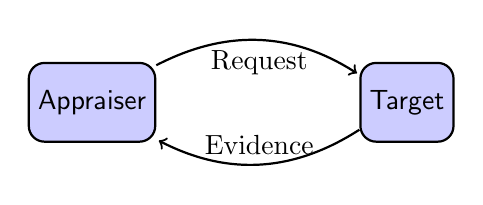
\begin{tikzpicture}[->,shorten >=1pt,auto,node distance=2.0cm,
  thick,main node/.style={rectangle,fill=blue!20,draw,
    font=\sffamily,minimum height=10mm,minimum width=10mm,rounded corners=2mm}]

  \node[main node] (app) {Appraiser};
  \node[main node] (tar) [node distance=4cm, right of=app] {Target};

  \path
  (app) edge[bend left] node[below] {Request} (tar)
  (tar) edge[bend left] node[above] {Evidence} (app)
  ;



  
\end{tikzpicture}
  \caption[Attestation architecture]{Remote attestation architecture showing an \emph{appraiser} \\ making an attestation request of a \emph{target}.}
  \label{fig:architecture-fig}
\end{figure}

In order to guide the development of the remote attestation architecture and its resulting systems, five guiding principles are established, as enumerated below \cite{prin_remote}. These principles are important to discuss as they motivate all remote attestation work. 
\begin{align*}
  1. &\text{Fresh Information} \\
  2. &\text{Comprehensive Information} \\
  3. &\text{Constrained Disclosure} \\ 
  4. &\text{Semantic Explicitness} \\
  5. &\text{Trustworthy Mechanism} 
\end{align*}

%% what more can I say here???

To understand how the principles can be realized, a definition of their meaning is necessary. First, the principle of fresh information states that the target must provide information about the current, running system. Secondly, the target must provide comprehensive information. This means the target must provide enough detail so that the appraiser can make an informed trust decision. Thirdly, the principle of constrained disclosure says that the communicating peers should be able to enforce their privacy standards. Specifically, the target should have some way of enforcing its privacy standards so as not to divulge sensitive information through the shared evidence. This idea can be implemented with a privacy policy, and is discussed in further in the following section \cite{flexible}. The fourth principle is the principle of semantic explicitness and it states the semantics should be logically defined. Finally, the principle of a trustworthy mechanism means that the underlying mechanism to establish trust is, in itself, trusted.   

Using these principles, we arrive at the current attestation framework. However, this framework does not allow for the target or appraiser to enforce their privacy requirements. As it stands, without any secure connection, the appraiser selects their desired measurement and the target must run it or it is automatically labeled untrustworthy. To combat this problem, and meet the peer's privacy needs, the idea of negotiation is introduced and explained in the following section. 

\subsection{Negotiation}

In order to meet the goals of comprehensive information and constrained disclosure, a negotiation routine must take place prior to attestation \cite{fritz}. The intent of negotiation is to allow the target and appraiser to agree on a measurement that simultaneously protects the target's privacy standards while ensuring the appraiser has enough information to make an informed trust decision. That is, the communicating peers must find a measurement that is comprehensive enough to satisfy the appraiser's need for comprehensive information and yet constrained enough to satisfy the target's need for constrained disclosure \cite{flexible}. Negotiation, as seen in Figure \ref{fig:sequence-fig}, allows the target and appraiser to meet these goals. 

\begin{figure}[hbtp]
  \centering 
  \begin{tikzpicture}[->,>=stealth',shorten >=1pt,auto,node distance=1.2cm,
  thick,main node/.style={rectangle,%%fill=blue!20,draw,
    font=\sffamily,minimum height=2mm,minimum width=2mm}]


  \node[main node] (RQ) {\textbullet};
  \node[main node] (SA) [below of=RQ] {\textbullet};
  \node[main node] (NM) [below of=SA] {\textbullet};
  \node[main node] (AM) [below of=NM] {\textbullet};
  \node[main node] (CP) [below of=AM] {\textbullet};
  \node[main node] (HW) [below of=CP] {\textbullet};
  \node[main node] (AP) [below of=HW] {\textbullet};
  \node[main node] (HWE) [node distance=3.5cm, right of=HW] {\textbullet};
  \node[main node] (CPE) [node distance=3.5cm, right of=CP] {\textbullet};
  \node[main node] (AME) [node distance=3.5cm, right of=AM] {\textbullet};
  \node[main node] (NME) [node distance=3.5cm, right of=NM] {\textbullet};
  \node[main node] (SAE) [node distance=3.5cm, right of=SA] {\textbullet};  
  \node[main node] (RQE) [node distance=3.5cm, right of=RQ] {\textbullet};  
  \node[main node] (IN) [node distance=1.0cm, above of=RQ] {Appraiser};
  \node[main node] (OUT) [node distance=1.0cm, above of=RQE] {Target};
    

  \path[every node/.style={font=\sffamily\small, fill=white,inner sep=1pt}]
    (RQ) edge node[above=1mm] {$SA$} (RQE)
    (SAE) edge node[above=1mm] {$SA$} (SA)
    (NM) edge node[above=1mm] {$R$} (NME)
    (AME) edge node[above=1mm] {$\langle P \rangle$} (AM)
    (CP) edge node[above=1mm] {$P$} (CPE)
    (HWE) edge node[above=1mm] {$E$} (HW)
    (RQE) edge node[right=1mm] {ISAKMP} (SAE)
    (SA) edge node[left=1mm] {ISAKMP} (NM)
    (NME) edge node[right=1mm] {Negotiation} (AME)
    (AM) edge node[left=1mm] {Selection} (CP)
    (CPE) edge node[right=1mm] {Attestation} (HWE)
    (HW) edge node[left=1mm] {Appraisal} (AP)
    ;
\end{tikzpicture}

%%% Local Variables: 
%%% mode: latex
%%% TeX-master: "negotiation20"
%%% End:

  \caption[Negotiation process]{The negotiation procedure \cite{fritz}.}
  \label{fig:sequence-fig}
%%\description{Attestation sequence.}
\end{figure}

The negotiation routine begins with the establishment of a security association (SA) through the Internet Security Association and Key Management Protocol (ISAKMP) \cite{ISAKMP}. That is, through ISAKMP, the situation, domain of interpretation, lifetime, and other situationally dependent criteria are established and recorded in a security association. Once that information is agreed upon, the appraiser sends the target a request. The request is one or more protocols the appraiser deems sufficient for attestation. It is situationally dependent and thus must take into consideration the information defined in the security association. Once the target receives the request, it applies its selection policy to generate a set of protocols that satisfy the request but do not expose sensitive information. This set, \emph{q}, is called the proposal. Again, the information the target deems private is situationally dependent and thus must take into consideration details presented in the security association. Once generated, the proposal $q$ is then sent back to the appraiser. Upon receiving the proposal, the appraiser can apply its selection policy to choose the best protocol for attestation. The resulting protocol, $p$, is then used in the attestation routine. 

\subsection{ISAKMP}

One essential piece of ensuring the negotiation routine is successful is proper understanding of the Internet Security Association and Key Management Protocol (ISAKMP). That is, this networking standard allows two remote parties to obtain a secure communication link through the establishment of security associations (SA) \cite{ISAKMP}. Each SA is unique to the communication context and can be conceptualized as a label of the agreed upon security services. Once instantiated, the SA protects subsequent traffic, thereby protecting all subsequent communications. 

In general, the ISAKMP communication procedure occurs in two phases where the goal of the first phase is to establish protection for the second phase \cite{ISAKMP}. To begin, the phase one procedure establishes the initial security association. This process is completed infrequently as it requires more networking resources and is therefore time and resource consuming \cite{ISAKMP}. However, once the first phase is complete, the basic SA is established and valid for a predetermined amount of time. With that, negotiations for the second phase can begin. During phase two, the initial SA is used to exchange key material as well as other security protocols. Phase two takes place frequently and is not time consuming.

Often, the actual information being negotiated in phase two is implementation dependent. For example, an IPSec implementation that uses ISAKMP to establish a secure communication link requires predetermined implementation dependent fields to be negotiated \cite{rfc_doi}. Some of these fields include the authentication header (AH) transform, the encapsulating security payload (ESP) transform, and the key exchange protocol. In most implementations, fields like hashing algorithm, signing algorithm, and lifetime of the security association are negotiated.  

%% To label each established SA, a local security parameter index (SPI) is used \cite{thesis}.

To situate this work within the networking stack, we present Figure \ref{stack} below. It can be seen that ISAKMP should be implemented on top of the IP layer but below the domain of interpretation (DOI) \cite{thesis}. In terms of an actual implementation of ISAKMP, the ISAKMP daemon is a user-level daemon that is registered with the operating system kernel \cite{thesis}. Existing SA's are stored in the kernel's engine and can be used by the system through standard security mechanisms.

\begin{figure}[hbtp]
  \begin{center}
    \includegraphics[scale=0.55]{stack} 
    \caption{ISAKMP in network stack \cite{handshake}}
    \label{stack}
  \end{center}
\end{figure}

We believe it is important to note that ISAKMP does exist in practice today as part of the IPSec implementation \cite{securing, design_IPsec}. However, in IPSec, ISAKMP and IKE are combined to meet the networking goals of confidentiality, integrity, and authenticity \cite{IKE_RFC}. The details of this are beyond our scope but we note that even though the framework was developed in the late 1990's, it is still useful today.

This simple overview may not provide enough detail to grasp the fundamentals of ISAKMP so as to understand how it can be used prior to remote attestation to aid in meeting the attestation principles. Therefore, in following subsections, additional information is presented. This includes information about exchange types, payload types, the domain of interpretation (DOI), and a motivating example of protocol exchanges. 

\subsubsection{Exchange Types}

Perhaps one of the most useful things about the ISAKMP framework is its flexibility. That is, to account for different communication scenarios, there are five types of exchanges: base exchange, identity protection exchange, authentication only exchange, aggressive exchange, and informational exchange \cite{ISAKMP}. Most exchanges are responsible for swapping keys and authentication information yet others serve as a means to transport single messages. It is the order of messages, the amount of messages, and the contents of the messages, that makes each exchange type unique. The outline for each exchange is presented in Appendix Figures \ref{fig:aggressive}, \ref{fig:auth}, \ref{fig:base}, \ref{fig:id_prot}, and \ref{fig:not} yet described in further detail below \cite{ISAKMP}. 

First, the base exchange communication routine occurs with the transmission of 4 messages. During this exchange, keying information and authentication information are sent together. Coupling this information reduces the number of round trips but does not protect the communicating parties identities. This is because identification information is exchanged before a shared secret is established. 

The identity protection exchange requires 6 messages total. The additional two messages allow keying information to be exchanged before the authentication information. This means this exchange can provide identity protection for the communicating parties as they can use the keying information as an established shared secret.

Next, the authentication only exchange operates with three messages where, as the name suggests, only the authentication information is exchanged.  This incurs less of a computational burden, as there is no need to compute keys. Yet, with the lack of keys, none of the subsequent information can be encrypted and therefore it is not protected.

The fourth exchange type is the aggressive exchange where all security relevant information is exchanged in one message. This limits the number of round trips. Yet, the downside is that the initiator only sends one proposal and transform payload, meaning the responder has no chance to negotiate future parameters. However, unlike the authentication only exchange, this exchange does transmit keys to allow for protection of future messages.

Finally, ISAKMP has an informational exchange in which only one message is transmitted to allow communicating peers to send a notification or delete message. The notification message can be used for tasks like key recovery \cite{recovery}. The delete message can be used to tell the responder to delete the security association. Either the party that initiated the connection or the party who responded may begin this type of exchange. Furthermore, the informational exchange may be sent at any time. 

\subsubsection{Payload Format}

Each exchange is composed of a series of one or more payloads \cite{ISAKMP}. To introduce a way to maintain state and allow for easier processing, each payload contains a fixed header. This header can be seen below in Figure \ref{fig:payload_header}. 

\begin{figure}[hbtp]
\centering
  \begin{bytefield}[bitwidth=1.1em]{32}
    \bitheader{0-31} \\
    \bitbox{32}{Initiator Cookie} \\
    \bitbox{32}{Responder Cookie} \\ 
    \bitbox{8}{Next Payload} & \bitbox{4}{MjVer} & \bitbox{4}{MnVer} & \bitbox{8}{Exchange Type} & \bitbox{8}{Flags} \\
    \bitbox{32}{Message ID} \\
    \bitbox{32}{Length}
\end{bytefield}
  \caption{The ISAKMP payload header \cite{ISAKMP}.}
  \label{fig:payload_header}
\end{figure}

For better understanding, the payload contents may require more description \cite{ISAKMP}. First, the initiator and responder cookies are used for the entity that initiated the security association and the one who responded to it, respectively. These values are unique to each communication scenario. As it sounds, the next payload field is a numeric value that is used to identify the next expected payload. The possible values, and their meanings, can be seen in Figure~\ref{fig:payloadtype}. Major and minor version are used to show compliance from the initiator and responder. They are automatically set to 1 for RFC 2408 (the ISAKMP communication routine) \cite{ISAKMP}. Following the minor version, the exchange type field is used to describe what type of exchange is occurring. The values for this can be visualized in Figure ~\ref{fig:exchangetype}. Next, the flag bits provide flexibility for three options: encryption bit, commit bit, and authentication only bit. If the encryption bit is set to 1 then all headers are encrypted. If the commit bit is set to 1 then the party that did not set the bit must wait for the information only exchange. Finally, if the authentication only bit is set to 1 then the information from the commit bit's information only exchange is not encrypted. The message ID field is used to identify protocol state. The last header is the length field which is implemented to indicate the total messages in octets. 


\begin{figure}
    \centering
    \begin{subfigure}[b]{0.4\textwidth}
        \centering
        \resizebox{\linewidth}{!}{\begin{tabular}{|c|c|}
\toprule
\textbf{Payload Type} & \textbf{Value}  \\
\midrule
Security Association (SA) & 1  \\
\midrule
Proposal (P) & 2 \\
\midrule
Transform (T) & 3 \\
\midrule
Key Exchange (KE) & 4 \\
\midrule
Identification (ID) & 5 \\
\midrule
Certificate (CERT) & 6 \\
\midrule
Certificate Request (CR) & 7 \\
\midrule
Hash (HASH) & 8 \\
\midrule
Signature (SIG) & 9 \\
\midrule
Nonce (NONCE) & 10 \\
\midrule
Notification (N) & 11 \\
\midrule
Delete (D) & 12 \\
\midrule
Vendor ID (VID) & 13 \\
\midrule
Private Use & 128-255 \\
\bottomrule
\end{tabular}} 
        % \begin{tabular}{|c|c|}
\toprule
\textbf{Payload Type} & \textbf{Value}  \\
\midrule
Security Association (SA) & 1  \\
\midrule
Proposal (P) & 2 \\
\midrule
Transform (T) & 3 \\
\midrule
Key Exchange (KE) & 4 \\
\midrule
Identification (ID) & 5 \\
\midrule
Certificate (CERT) & 6 \\
\midrule
Certificate Request (CR) & 7 \\
\midrule
Hash (HASH) & 8 \\
\midrule
Signature (SIG) & 9 \\
\midrule
Nonce (NONCE) & 10 \\
\midrule
Notification (N) & 11 \\
\midrule
Delete (D) & 12 \\
\midrule
Vendor ID (VID) & 13 \\
\midrule
Private Use & 128-255 \\
\bottomrule
\end{tabular}
        \caption{Payload Type Values \cite{ISAKMP}}
        \label{fig:payloadtype}
    \end{subfigure}
    \begin{subfigure}[b]{0.4\textwidth}
        \centering
        \resizebox{\linewidth}{!}{\begin{tabular}{|c|c|}
\toprule
\textbf{Exchange Type} & \textbf{Value}  \\
\midrule
NONE & 0  \\
\midrule
Base & 1  \\
\midrule
Identity Protection & 2 \\
\midrule
Authentication Only & 3 \\
\midrule
Aggressive & 4 \\
\midrule
Informational & 5 \\
\midrule
ISAKMP Future Use & 6-31 \\
\midrule
DOI Specific Use & 32-239 \\
\midrule
Private Use & 240-255 \\
\bottomrule
\end{tabular}}
        % \begin{tabular}{|c|c|}
\toprule
\textbf{Exchange Type} & \textbf{Value}  \\
\midrule
NONE & 0  \\
\midrule
Base & 1  \\
\midrule
Identity Protection & 2 \\
\midrule
Authentication Only & 3 \\
\midrule
Aggressive & 4 \\
\midrule
Informational & 5 \\
\midrule
ISAKMP Future Use & 6-31 \\
\midrule
DOI Specific Use & 32-239 \\
\midrule
Private Use & 240-255 \\
\bottomrule
\end{tabular}
        \caption{Exchange Type Values \cite{ISAKMP}}
        \label{fig:exchangetype}
    \end{subfigure} 
    \caption{Values for Payloads.}
\end{figure}

\newpage
\subsubsection{Domain of Interpretation}

At its core, the goal of ISAKMP is to establish security associations (SA). One key component of the SA is the domain of interpretation (DOI). Within the DOI, communicating peers can group security related properties so that the peers can negotiate about their requirements \cite{rfc_doi}. In summary, the DOI is designed to:

\begin{enumerate}
    \squash
    \item define naming schemes 
    \item define the interpretation of the situation field 
    \item define useful security policies 
\end{enumerate}

In implementation, the negotiated domain of interpretation is located in the security association payload \cite{ISAKMP}. To house such information, there is one security association payload per communication context. As seen in Figure \ref{fig:SA_pay}, the SA payload includes the DOI and the situation. The situation field describes the context of communication so that the peers can make informed policy decisions when negotiating during the establishment of the SA \cite{rfc_doi}. 

\begin{figure}[hbtp]
\centering
  \begin{bytefield}[bitwidth=1.1em]{32}
    \bitheader{0-31} \\
    \bitbox{8}{Next Payload} &
    \bitbox{8}{Reserved} & 
    \bitbox{16}{Payload Length} \\
    \bitbox{32}{Domain of Interpretation (DOI)} \\
    \wordbox[tlr]{1}{Situation} \\
    \wordbox[blr]{1}{$\cdots$} \\
\end{bytefield}
  \caption{Security Association Payload. \cite{ISAKMP}}
  \label{fig:SA_pay}
\end{figure}

One example of an implementation of the DOI occurs when using ISAKMP for IPSec. In this case, we observe the possible values for the situation to motivate its use. That is, the situation is realized as an octet bit mask with the following options: identity only, secrecy, and integrity \cite{rfc_doi}. For the identity only situation, the DOI can be recognized in an associated identification payload. For secrecy, the SA should be negotiated in an environment that requires secrecy. And, for integrity, the SA negotiation procedure should occur in an environment that requires integrity. This is simply one example that motivates the need and use of the situation field.

\subsubsection{Protocol Exchange}

To establish a security association, one or more payloads will be transmitted between the communicating peers \cite{ISAKMP}. Specifically, there must be a single SA payload, which contains information describing the domain of interpretation and the situation as seen in Section 2.3.3. Following the SA payload, there maybe one or more proposal payloads. Each proposal payload is associated with a transform payload. The transform payload contains the specific security mechanisms to be used in the protocol. 

To better understand this, consider the example in Figure \ref{fig:pay_ex}. As previously stated, the payload begins with the SA payload which contains the DOI and situation. The subsequent payloads contain two options for the resulting protection suite. The first option is protocol 1 with transform 1 and 2. This protocol is ESP and the transforms are 3DES and DES, respectively. The second proposed protocol (Prop1 Prot2) is the AH protocol with the transform SHA. With that, the responder chooses the resulting protection suite which will be either 3DES and SHA or DES and SHA. 

\begin{figure}[hbtp]
\centering
  \begin{bytefield}[bitwidth=1.1em]{32}
    \bitheader{0-31} \\
    \begin{rightwordgroup}{SA \\  Pay}
        \bitbox{8}{NP = Nonce} & \bitbox{8}{Reserved} & \bitbox{16}{Payload Length} \\
        \bitbox{32}{Domain of Interpretation (DOI)} \\
        \bitbox{32}{Situation}
    \end{rightwordgroup} \\
    \begin{rightwordgroup} {Prop 1 \\ Prot 1}
        \bitbox{8}{NP = Proposal} & \bitbox{8}{Reserved} & \bitbox{16}{Payload Length} \\
        \bitbox{8}{Proposal \# = 1} & \bitbox{8}{Protocol-Id} & \bitbox{8}{SPI Size} &\bitbox{8}{\# of Trans. = 2} \\
        \bitbox{32}{SPI (Variable)}
    \end{rightwordgroup} \\
    \begin{rightwordgroup} {Tran 1}
        \bitbox{8}{NP = Transform} & \bitbox{8}{Reserved} & \bitbox{16}{Payload Length} \\
        \bitbox{8}{Transform \# = 1} & \bitbox{8}{Transform ID} & \bitbox{16}{Reserved2}  \\
        \bitbox{32}{SA Attributes (3DES)}
    \end{rightwordgroup} \\
    \begin{rightwordgroup} {Tran 2}
        \bitbox{8}{NP = 0} & \bitbox{8}{Reserved} & \bitbox{16}{Payload Length} \\
        \bitbox{8}{Transform \# = 2} & \bitbox{8}{Transform ID} & \bitbox{16}{Reserved2}  \\
        \bitbox{32}{SA Attributes (DES) }
    \end{rightwordgroup} \\
    \begin{rightwordgroup} {Prop 1 \\ Prot 2}
        \bitbox{8}{NP = 0} & \bitbox{8}{Reserved} & \bitbox{16}{Payload Length} \\
        \bitbox{8}{Proposal \# = 1} & \bitbox{8}{Protocol-Id} & \bitbox{8}{SPI Size} &\bitbox{8}{\# of Trans. = 1} \\
        \bitbox{32}{SPI (Variable)}
    \end{rightwordgroup} \\
    \begin{rightwordgroup} {Tran 1}
        \bitbox{8}{NP = 0} & \bitbox{8}{Reserved} & \bitbox{16}{Payload Length} \\
        \bitbox{8}{Transform \# = 1} & \bitbox{8}{Transform ID} & \bitbox{16}{Reserved2}  \\
        \bitbox{32}{SA Attributes (SHA) }
    \end{rightwordgroup} \\

\end{bytefield}
  \caption{Security Association establishment example \cite{ISAKMP}.}
  \label{fig:pay_ex}
\end{figure}

Once the responder chooses the resulting protection suite, the security association is established and used for subsequent communications. Showcasing this simple example highlights the flexibility of ISAKMP as many different proposals can be made to account for a variety of situations. 

\subsection{Motivation for this work}
Currently, the remote attestation framework neglects to describe the mechanism for establishing a secure connection prior to the attestation routine. Authors who typically write about the attestation work tend to assume the connection away, stating that it already exists and further communication is taking place under the pretense of the secure agreement \cite{ietf-reference-interaction-models-04}. In this work, we present a mechanism for creating a secure connection while describing how it can be implemented to capture the situational needs of the attestation framework.    

\section{The Use of ISAKMP for Secure Connections}

There is little existing work that describes the networking requirements to establish a secure connection prior to remote attestation \cite{ietf-reference-interaction-models-04}. As previously stated, we choose to implement ISAKMP to meet this need. Therefore, in this section, we discuss a practical ISAKMP exchange type for remote attestation as well as define accompanying ISAKMP fields to provide necessary contextual information for the success of the attestation routine. 

%% need to discuss WHY isakmp 

When implementing ISAKMP, first we must to choose an exchange type. Perhaps the best fit for attestation is the Identity Protection Exchange so as to ensure that the identity of the target and appraiser are not vulnerable to third party attackers lingering on the network. Because we would like to mitigate attacks, the Identity Protection Exchange type is most effective, as the transmitted keys can be used to protect subsequent traffic. This can be observed below in Figure \ref{fig:id_prot_fig}.  

\begin{figure}[hbtp]
\centering
\tcbox{
  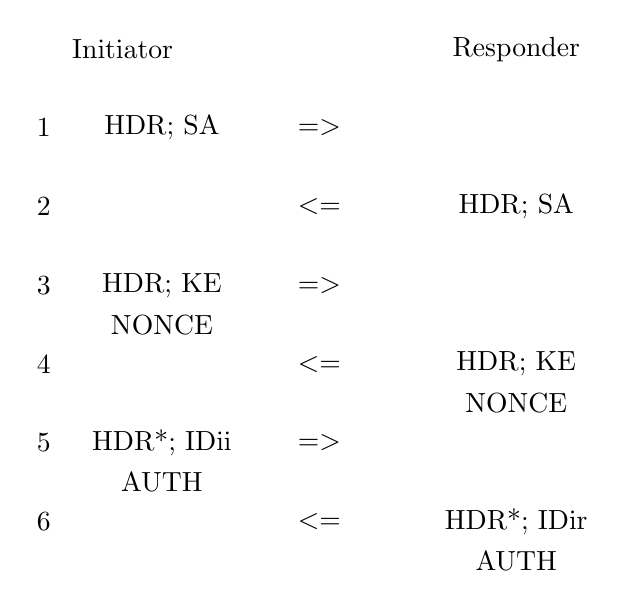
\begin{tikzpicture}

  
    %%[->,>=stealth',shorten >=1pt,auto,node distance=1.2cm,
    %%  thick, main node/.style={rectangle}]
      
      %%fill=blue!20,draw,font=\sffamily,minimum height=2mm,minimum width=2mm}]
        
      \node (Number) {};  
      \node(Initiator) [right of=Number] {Initiator};
      \node(Direction) [node distance=2.5cm, right of=Initiator] {};
      \node(Responder) [node distance=2.5cm, right of=Direction] {Responder};
      
      \node (ONE) [below of=Number] {1};
      \node (TWO) [below of=ONE] {2};
      \node (THREE) [below of=TWO] {3};
      \node (FOUR) [below of=THREE] {4};
      \node (FIVE) [below of=FOUR] {5};
      \node (SIX) [below of=FIVE] {6};
  
  
      \node (A1) [below of=Direction] {$=>$}; S
      \node (A2) [below of=A1] {$<=$}; 
      \node (A3) [below of=A2] {$=>$}; 
      \node (A4) [below of=A3] {$<=$};
      \node (A5) [below of=A4] {$=>$};
      \node (A6) [below of=A5] {$<=$}; 
        
      \node (I1) [node distance=1.5cm, right of=ONE] {HDR; SA};    
      %%\node (I1b) [node distance=0.5cm, below of=I1] {NONCE};   
      
      \node (R2) [node distance=6cm, right of=TWO] {HDR; SA};
      
      \node (I3) [node distance=1.5cm,right of=THREE] {HDR; KE}; 
      \node (I3b) [node distance=0.5cm, below of=I3] {NONCE};
      
      \node (R4) [node distance=6cm,right of=FOUR] {HDR; KE}; 
      \node (R4b) [node distance=0.5cm, below of=R4] {NONCE};

      \node (I5) [node distance=1.5cm,right of=FIVE] {HDR*; IDii}; 
      \node (I5b) [node distance=0.5cm, below of=I5] {AUTH};

      \node (R6) [node distance=6cm,right of=SIX] {HDR*; IDir}; 
      \node (R6b) [node distance=0.5cm, below of=R6] {AUTH};
      
  
    \end{tikzpicture}
  }
  \caption[Base process]{Identity Protection Exchange. Figure adopted from RFC 2408\cite{ISAKMP}.}
  \label{fig:id_prot_fig}
\end{figure}

It is important to understand that ISAKMP is not only useful for setting up a secure communication link but also for realizing situationally dependent information that impacts the negotiation routine. That is, the goal of negotiation is to obtain a sufficient measurement for attestation. This measurement is often situationally dependent meaning there must be some way to determine the situational needs prior to negotiation. To do this, the flexible nature of ISAKMP can be exploited to define valuable information. 


With each exchange, there are a number of mutable payloads. This means parameters that are specifically useful for negotiation can be included by using the predetermined, provided payloads, like the ones seen in Figure \ref{fig:payloadtype} or using the private use payloads. In either case, ensuring the situationally dependent information is exchanged is necessary for the success of remote attestation. With that, we realize the following information must be determined through ISAKMP, as listed below: 

\begin{itemize}
\squash
    \item Identities
    \item Situation
    \item Hashing algorithm
    \item Signing algorithm
    \item Lifetime
\end{itemize}

%% time to live counter ttl 
%% raccoon implementation 

First, identities must be determined prior to remote attestation. The peers must be aware of who they are engaging with because both the target and appraiser must uphold the goal of constrained disclosure. By providing this awareness through the identity field, the peers can then determine what policies are necessary to protect their information. The identities are also necessary to establish the situation, as discussed next. With any ISAKMP exchange, the identities are shared in the identification payload. Therefore, the ISAKMP framework already accounts for the transfer of identification information. 

Following the identification information, the situation is needed to describe the context of communication as the negotiation procedure cannot be successful without such information. This contextual information can be realized with a label in the situation field. To motivate this, consider one such situation where attestation must be performed quickly. Because of this label in the situation field, negotiation may produce a simple measurement that the target can use to swiftly generate evidence. On the other hand, if a more robust measurement is required, the situation label could reflect that need. While the situation field does exist in ISAKMP, the values are implementation dependent and defined in the coming sections. 

Next, both the hashing and signing algorithms must be agreed upon by the target and appraiser as they are used in the attestation process. Both of these have payload fields associated with them in the ISAKMP framework. Therefore, it will be easy to implement these features. 

Finally, the lifetime component is traditionally used to communicate the duration the SA is valid. However, here, the lifetime is implemented in a  separate field to convey how long the results of remote attestation procedure should be valid. In other words, the appraiser must state the duration of the trust decision as once expired, it is no longer valid. By having this field within the ISAKMP communication routine, we can meet the remote attestation goal of fresh information as once this value times out the information is no longer fresh. For implementation, ISAKMP is equipped with a lifetime payload which can be copied for our purposes.

Each one of these fields has a set of values which they can employ, as seen in Figure \ref{fig:values}. To start, the identity can either be $T$ or $A$ to represent the target or the appraiser. There may be additional identification information needed but that is abstracted to these values for now. Next, the situation can be one of three values. In most cases, the situation is normal, meaning attestation should proceed as designed. However, the situation may be dangerous meaning there is no room for negotiation of security parameters or other timely considerations. The connection must be established swiftly so that the trust decision can be made as quick as possible. The third option for situational values is the extended value. In this case, the appraiser wants a more comprehensive view of the target  so the situation reflects the desire for a more detailed measurement. Following the situational values, there are fields for the hashing and signing algorithms. For hashing algorithms, these values may be one like MD5, SHA-256, or others. For signing algorithms, these values may be RSA, DSA, or any others. These values reflect current, acceptable algorithms. The last defined field is the lifetime component which depicts the length the trust decision is valid. It may be until the connection ends, every 5 minutes, every 5 hours, or some eluded amount of time.

\begin{figure}[hbtp]
    \centering
    \begin{tabular}{|c|c|}
\toprule
\textbf{Field} & \textbf{Possible Values}  \\
\midrule
Identities &  \{$A$, $T$\} \\
\midrule
Situation &  \{Extended, Normal, Dangerous\} \\
\midrule
Hashing algorithm &  \{SHA-256, MD5 ... \} \\
\midrule
Signing algorithm & \{RSA, DSA ... \} \\
\midrule
Lifetime &  \{ t $|$ $ t > 0 $ \} $\cup$ \{terminating connection\} \\
\bottomrule
\end{tabular}
    \caption{Possible values for each field in the security association. }
    \label{fig:values}
\end{figure}

Because of the flexible nature of ISAKMP, we can easily fit these values into payloads to contextualize the communication. This is useful to meet the principles of remote attestation and also the negotiation requirements. 

%\section{Negotiating Properties}
\section{Examples}

%% different nodes for attestation but 1-1 then  
As previously discussed, ISAKMP is used to establish a security association prior to negotiation and remote attestation. We determined that the identities, situation, hashing algorithm, signing algorithm, and lifetime need to be negotiated and presented in the security association. To motivate the choice of these particular fields, we present some provoking examples. These examples fall into three categories representing three different situations where remote attestation may be useful. That is, a one-on-one attestation, a one-to-many attestation, and a many-to-one attestation.   

For the first situation, consider the case of attesting to the state of the bank's software as a one-to-one example. In this case, the situation is normal as the attestation routine is not hurried due to some threat; it can operate normally. The values for hashing and signing here, and in all following examples, are extraneous. An interesting feature, in this case, is the lifetime value as we must capture the fact that the trust decision should be valid until the connection terminates. Logically, this is because when you establish connection to your bank's server, you want to be able to do tasks without being logged out. But, once you do log out, you need to be reassessed for trust. The values for all parameters can be observed in the table below. 

\begin{center}
    \begin{tabular}{ | m{15em} | m{15em}| } 
      \hline
      Identities & $T$ , $A$ \\ 
      \hline
      Lifetime & Terminating connection \\ 
      \hline
      Hashing algorithm & MD5 \\
      \hline
      Signing algorithm & RSA \\
      \hline
      Situation & Normal \\
      \hline
    \end{tabular}
\end{center}

For the second situation, consider the case where you, as a user from your home network, would like to a join a cooperate network. This one-to-many case requires you to attest to the state of the many cooperate servers. You may be interfacing with one server but that may just be one of many on the network. In order to provide your system with a complete understanding of the cooperate network's state, the attestation protocol is meticulous and therefore the situation is extended. Again, the lifetime of the trust decision expires upon terminating the communication as once you log off the cooperate network, the trust decision is no longer valid. The values for all parameters can be seen in the table below. 

\begin{center}
    \begin{tabular}{ | m{15em} | m{15em}| } 
      \hline
      Identities & $T , A$ \\ 
      \hline
      Lifetime & Terminating connection \\ 
      \hline
      Hashing algorithm & MD5 \\
      \hline
      Signing algorithm & RSA \\
      \hline
      Situation & Extended \\
      \hline
    \end{tabular}
\end{center}

Thirdly, consider the same situation as example two but in reverse. This time, the cooperate network would like to attest to your state before you join the infrastructure. Instead of having an extended attestation situation, since the target is only one communicating peer, it is normal again. There is nothing dangerous or extended about the session, it is just many servers trying to asses the state of one device to make a trust decision. The values for the various fields can be visualized in the table below. 

\begin{center}
    \begin{tabular}{ | m{15em} | m{15em}| } 
      \hline
      Identities & $T , A$ \\ 
      \hline
      Lifetime & Terminating connection \\ 
      \hline
      Hashing algorithm & MD5 \\
      \hline
      Signing algorithm & RSA \\
      \hline
      Situation & Normal \\
      \hline
    \end{tabular}
\end{center}

Hopefully these examples help to motivate the need for ISAKMP prior to negotiation and remote attestation. That is, these additionally proposed fields already exist within the ISAKMP framework as various payloads. With the flexible nature of the ISAKMP framework, we can morph them to fit the needs for negotiation and remote attestation to produce useful contextual information.

\section{Conclusion}

In this report, we have shown why ISAKMP may be an advantageous addition to the remote attestation routine. At first glance, ISAKMP can be applied to institute a secure connection prior to remote attestation through the establishment of security associations. Yet, its flexible nature also allows the framework to establish situationally dependent details. Taking this into consideration, we introduce the required identity, lifetime, hashing algorithm, signing algorithm, and situation payloads to the ISAKMP routine to situate the communication context. This allows the target to meet their goals of constrained disclosure as now, because of the identity and situation fields, they have an understanding of what information is considered private. Similarly, because of the contextual details the appraiser can speculate about what it means to have comprehensive information. Thus, by introducing this idea of implementing ISAKMP prior to remote attestation we not only set up a secure networking connection but also help meet the principles of attestation.   

\printbibliography


\section{Appendix}

\begin{figure}[hbtp]
\centering
\tcbox{
  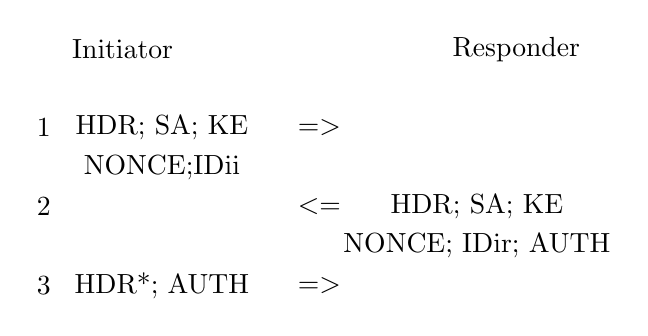
\begin{tikzpicture}
  
  %%fill=blue!20,draw,font=\sffamily,minimum height=2mm,minimum width=2mm}]
    
  \node (Number) {};  
  \node (Initiator) [right of=Number] {Initiator};
  \node (Direction) [node distance=2.5cm, right of=Initiator] {};
  \node (Responder) [node distance=2.5cm, right of=Direction] {Responder};
  
  \node (ONE) [below of=Number] {1};
  \node (TWO) [below of=ONE] {2};
  \node (THREE) [below of=TWO] {3};
  
  \node (A1) [below of=Direction] {$=>$}; S
  \node (A2) [below of=A1] {$<=$}; 
  \node (A3) [below of=A2] {$=>$}; 
    
  \node (I1) [node distance=1.5cm, right of=ONE] {HDR; SA; KE};    
  \node (I1b) [node distance=0.5cm, below of=I1] {NONCE;IDii};   
  
  \node (R2) [node distance=5.5cm, right of=TWO] {HDR; SA; KE};
  \node (R2b) [node distance=0.5cm, below of=R2] {NONCE; IDir; AUTH}; 
  
  \node (I3) [node distance=1.5cm,right of=THREE] {HDR*; AUTH}; 
  
  
  
\end{tikzpicture}
  }
  \caption{Aggressive Exchange \cite{ISAKMP}.}
  \label{fig:aggressive}
\end{figure}

\begin{figure}[hbtp]
\centering
\tcbox{
  \input{exchange_types_all/auth}
  }
  \caption{Authentication Exchange \cite{ISAKMP}.}
  \label{fig:auth}
\end{figure}

\begin{figure}[hbtp]
\centering
\tcbox{
  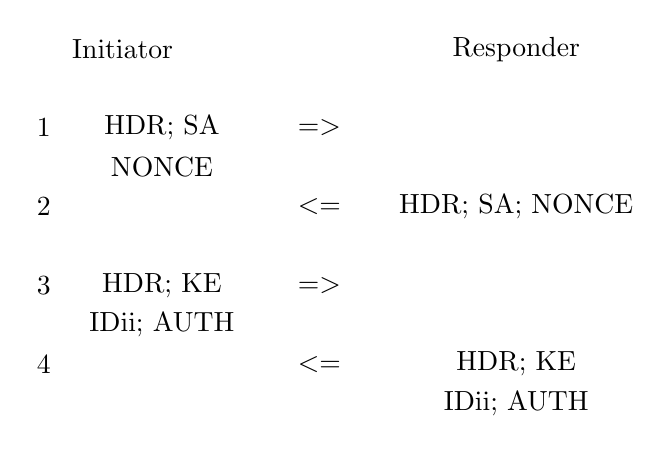
\begin{tikzpicture}
  
  %%[->,>=stealth',shorten >=1pt,auto,node distance=1.2cm,
  %%  thick, main node/.style={rectangle}]
    
    %%fill=blue!20,draw,font=\sffamily,minimum height=2mm,minimum width=2mm}]
      
    \node (Number) {};  
    \node(Initiator) [right of=Number] {Initiator};
    \node(Direction) [node distance=2.5cm, right of=Initiator] {};
    \node(Responder) [node distance=2.5cm, right of=Direction] {Responder};
    
    \node (ONE) [below of=Number] {1};
    \node (TWO) [below of=ONE] {2};
    \node (THREE) [below of=TWO] {3};
    \node (FOUR) [below of=THREE] {4};


    \node (A1) [below of=Direction] {$=>$}; S
    \node (A2) [below of=A1] {$<=$}; 
    \node (A3) [below of=A2] {$=>$}; 
    \node (A4) [below of=A3] {$<=$}; 
      
    \node (I1) [node distance=1.5cm,right of=ONE] {HDR; SA};    
    \node (I1b) [node distance=0.5cm, below of=I1] {NONCE};   
    
    \node (R2) [node distance=6cm, right of=TWO] {HDR; SA; NONCE};
    
    \node (I3) [node distance=1.5cm,right of=THREE] {HDR; KE}; 
    \node (I3b) [node distance=0.5cm, below of=I3] {IDii; AUTH};
    
    \node (R4) [node distance=6cm,right of=FOUR] {HDR; KE}; 
    \node (R4b) [node distance=0.5cm, below of=R4] {IDii; AUTH};

  \end{tikzpicture}
  }
  \caption{Base Exchange \cite{ISAKMP}.}
  \label{fig:base}
\end{figure}


\begin{figure}[hbtp]
\centering
\tcbox{
  \input{exchange_types_all/id_protect}
  }
  \caption{Identity Protection Exchange \cite{ISAKMP}.}
  \label{fig:id_prot}
\end{figure}

\begin{figure}[hbtp]
\centering
\tcbox{
  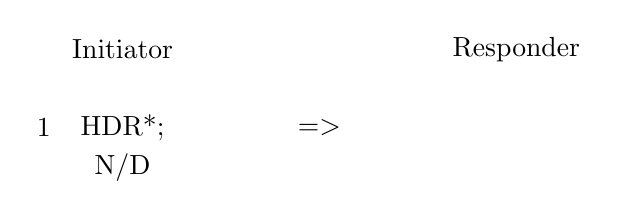
\begin{tikzpicture}
  
    %%[->,>=stealth',shorten >=1pt,auto,node distance=1.2cm,
    %%  thick, main node/.style={rectangle}]
      
      %%fill=blue!20,draw,font=\sffamily,minimum height=2mm,minimum width=2mm}]
        
      \node (Number) {};  
      \node(Initiator) [right of=Number] {Initiator};
      \node(Direction) [node distance=2.5cm, right of=Initiator] {};
      \node(Responder) [node distance=2.5cm, right of=Direction] {Responder};
      
      \node (ONE) [below of=Number] {1};

      \node (A1) [below of=Direction] {$=>$}; S
     
        
      \node (I1) [right of=ONE] {HDR*;};    
      \node (I1b) [node distance=0.5cm, below of=I1] {N/D};   
  
    \end{tikzpicture}
  }
  \caption{Notification Exchange \cite{ISAKMP}.}
  \label{fig:not}
\end{figure}

\end{document}